\documentclass[11pt,a4paper]{article}

\usepackage[utf8]{inputenc}
\usepackage[T1]{fontenc}
\usepackage[french]{babel}
\usepackage{lmodern}
\usepackage[margin=2.4cm]{geometry}
\usepackage{graphicx}
\usepackage{booktabs}
\usepackage{array}
\usepackage{xcolor}
\usepackage{colortbl}
\usepackage{tcolorbox}
\usepackage{enumitem}
\usepackage{hyperref}
\usepackage{fancyhdr}
\usepackage{titlesec}

\definecolor{primary}{RGB}{31,71,120}
\definecolor{softgrey}{RGB}{242,244,247}
\definecolor{danger}{RGB}{176,42,42}

\hypersetup{colorlinks=true,linkcolor=primary,urlcolor=primary}

\titleformat{\section}{\color{primary}\Large\bfseries}{\thesection.}{0.6em}{}
\titleformat{\subsection}{\color{primary}\large\bfseries}{\thesubsection.}{0.5em}{}

\pagestyle{fancy}
\fancyhf{}
\lhead{\small Assistant radiologue virtuel responsable}
\rhead{\small EFREI --- 2025-2026}
\cfoot{\thepage}
\renewcommand{\headrulewidth}{0.4pt}

\newtcolorbox{warnbox}{colback=danger!8,colframe=danger,boxrule=0.8pt,arc=2pt,left=6pt,right=6pt,top=4pt,bottom=4pt}
\newtcolorbox{keybox}{colback=softgrey,colframe=primary,boxrule=0.6pt,arc=2pt,left=6pt,right=6pt,top=4pt,bottom=4pt}

\begin{document}

\begin{titlepage}
\centering
\vspace*{2cm}
{\color{primary}\Huge\bfseries Assistant radiologue virtuel responsable\par}
\vspace{0.6cm}
{\Large Prototype pédagogique d'IA multimodale pour l'analyse prudente\\de radiographies thoraciques\par}
\vspace{1.5cm}
{\large\bfseries Rapport final\par}
\vspace{2cm}
\begin{keybox}
\centering
\textbf{Filière} Data / Intelligence artificielle --- Solution Delivery\\[4pt]
\textbf{École} EFREI Paris\\[4pt]
\textbf{Année académique} 2025-2026\\[4pt]
\textbf{Modèle évalué} \texttt{google/medgemma-4b-it} (4-bit, QLoRA-ready)
\end{keybox}
\vspace{1.5cm}
\begin{warnbox}
\centering\small
\textbf{Position non clinique.} Ce prototype n'est pas un dispositif médical. Il ne doit jamais
être utilisé pour diagnostiquer, trier ou orienter un patient. Toute sortie est un résultat
expérimental devant être vérifié par un professionnel qualifié.
\end{warnbox}
\vfill
{\small Prototype pédagogique. Non destiné au diagnostic. Validation par un professionnel qualifié requise.\par}
\end{titlepage}

\tableofcontents
\newpage

\section{Périmètre et jeu de données}

\subsection{Objectif et périmètre}
Le projet développe une application web qui reçoit une radiographie thoracique frontale et
retourne une sortie JSON structurée : qualité de l'image, classe prédite parmi
\{\texttt{normal}, \texttt{suspected\_opacity}, \texttt{uncertain}\}, confiance, observations
visuelles, justification courte, limites et avertissement obligatoire. Le projet ne vise pas le
diagnostic : il vise l'apprentissage d'une démarche d'ingénierie responsable --- périmètre
restreint, baseline reproductible, métriques, journaux, garde-fous et limites documentées.

\subsection{Jeu de données}
L'évaluation porte sur un jeu synthétique de 30 images, réparties de façon équilibrée
(10 \texttt{normal}, 10 \texttt{suspected\_opacity}, 10 \texttt{uncertain}). Ces images sont
générées procéduralement (\texttt{source = synthetic\_toy}) et ne contiennent aucune donnée
patient réelle. Le choix des données synthétiques est explicitement autorisé par le cahier des
charges (\emph{« Synthétiques ou publiques, autorisées et dé-identifiées »}).

\begin{keybox}
\textbf{Limite fondamentale assumée.} Les images ne sont pas de vraies radiographies. Les scores
rapportés mesurent le comportement du \emph{pipeline} et la \emph{sensibilité aux prompts}, non
une performance clinique. Un score élevé sur ce jeu ne constitue en aucun cas une validation
médicale.
\end{keybox}

\section{Architecture et baseline reproductible}

\subsection{Chaîne de traitement}
La chaîne est volontairement découplée pour rester exécutable sans GPU en démonstration :
\[
\text{Image} \rightarrow \text{Preprocessing} \rightarrow \text{MedGemma 4B (hors-ligne, 4-bit)} \rightarrow \text{Guardrails} \rightarrow \text{JSON} \rightarrow \text{UI / SQLite}
\]
L'inférence lourde du modèle multimodal est exécutée \emph{une seule fois} en traitement par lot
sur GPU (Colab T4, quantification 4-bit via BitsAndBytes). Les prédictions sont mises en cache
(\texttt{eval/cached\_predictions/*.json}). L'API FastAPI, les interfaces Streamlit/Gradio et le
protocole d'évaluation ne rechargent jamais le modèle : ils lisent le cache. Ce découplage rend
toute la surface évaluée reproductible sur CPU et déterministe (décodage glouton,
\texttt{do\_sample=False}).

\subsection{Modèle et baseline}
La baseline applique un prompt simple à MedGemma 4B. Sur le jeu synthétique, elle atteint une
exactitude de \textbf{80,0\,\%} et un macro-F1 de \textbf{78,0\,\%}, avec 100\,\% de sorties JSON
valides et 100\,\% d'avertissements présents. Sa faiblesse principale est une sensibilité aux
opacités de seulement \textbf{40\,\%} (6 opacités sur 10 classées à tort \texttt{normal}).

\section{Amélioration mesurée : itération des prompts}

Le c\oe ur de ce travail est une itération d'ingénierie \emph{mesurée} à chaque étape. Trois
variantes de prompt ont été comparées à la baseline sur les mêmes 30 images. Le résultat central
est qu'une formulation « prudente » plausible peut rendre le système \emph{plus dangereux} : seule
la mesure le révèle.

\begin{table}[h]
\centering
\renewcommand{\arraystretch}{1.3}
\begin{tabular}{lccccc}
\toprule
\textbf{Version} & \textbf{Exactitude} & \textbf{Macro-F1} & \textbf{Sensib. opacité} & \textbf{Faux négatifs} & \textbf{Taux incert.}\\
\midrule
Baseline & 80,0\,\% & 78,0\,\% & 40\,\% & 6 & 33,3\,\%\\
\rowcolor{danger!8} v1 (strict) & 66,7\,\% & 55,6\,\% & 0\,\% & 10 & 33,3\,\%\\
\rowcolor{danger!8} v2 (sur-prudent) & 36,7\,\% & 25,6\,\% & 100\,\% & 0 & 33,3\,\%\\
\rowcolor{primary!12} \textbf{v3 (équilibré)} & \textbf{86,7\,\%} & \textbf{86,9\,\%} & \textbf{90\,\%} & \textbf{1} & 26,7\,\%\\
\bottomrule
\end{tabular}
\caption{Comparaison des quatre stratégies de prompt (30 cas synthétiques).}
\end{table}

\begin{figure}[h]
\centering
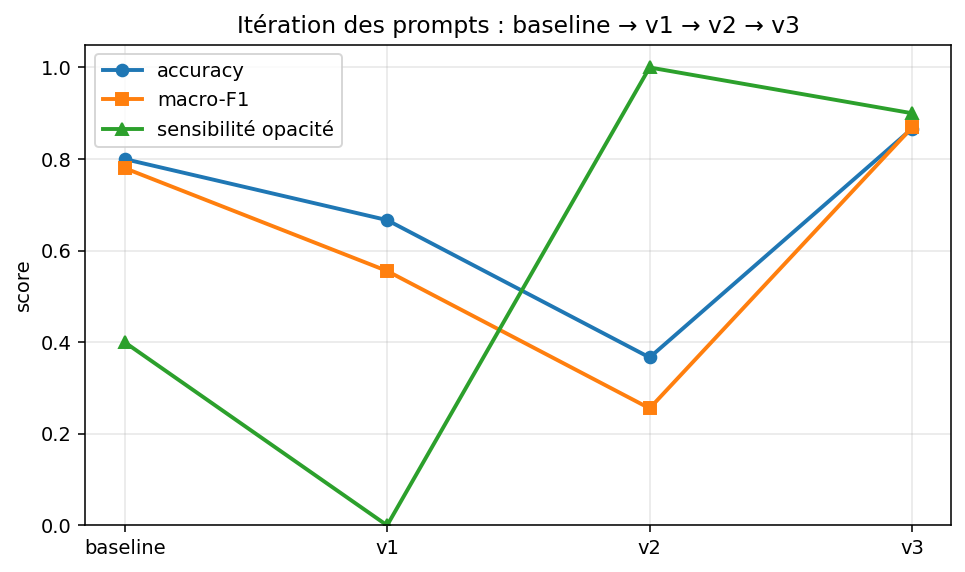
\includegraphics[width=\textwidth]{figures/metric_trajectory.png}
\caption{Trajectoire des métriques au fil de l'itération. La v3 domine la baseline sur tous les axes.}
\end{figure}

\subsection{v1 --- trop permissif : faux négatifs surconfiants}
Le prompt v1 ajoutait une consigne stricte invitant à considérer qu'une anomalie apparente
pouvait résulter d'un artefact (projection, rotation, exposition). L'intention était la prudence.
L'effet mesuré fut l'inverse : le modèle a utilisé cette consigne pour \emph{écarter} les
opacités et conclure à un \texttt{normal} confiant. Sur les cas concernés, la confiance est
\emph{montée} de 0,70 à 0,95 tout en devenant fausse --- une miscalibration caractéristique. La
sensibilité aux opacités s'est effondrée à 0\,\% (10 faux négatifs sur 10), soit l'erreur la plus
dangereuse en contexte de dépistage.

\subsection{v2 --- trop strict : le détecteur qui « crie au loup »}
En réaction, le prompt v2 imposait un biais de sécurité fort (« ne jamais rater une anomalie »).
La sensibilité aux opacités atteint alors 100\,\% et les faux négatifs tombent à 0, mais au prix
d'un effondrement de la précision : le modèle classe presque toutes les images comme
\texttt{suspected\_opacity} ou \texttt{uncertain}, y compris les 10 images réellement
\texttt{normal} (précision \texttt{normal} nulle). Un détecteur qui alarme sur tout est aussi
inutile qu'un détecteur qui n'alarme jamais.

\subsection{v3 --- l'équilibre : diagnostic puis correction}
Le prompt v3 applique des règles \emph{symétriques} : le doute est routé vers \texttt{uncertain}
(jamais vers un \texttt{normal} confiant), mais une image manifestement saine peut redevenir
\texttt{normal}. Une anomalie visible ne peut plus être « expliquée » en \texttt{normal}, sans que
cela impose pour autant de tout signaler. Résultat : la v3 \textbf{dépasse la baseline sur toutes
les métriques} --- exactitude 86,7\,\%, macro-F1 86,9\,\% --- tout en ramenant les faux négatifs
de 6 à 1 et la sensibilité aux opacités de 40\,\% à 90\,\%.

\begin{figure}[h]
\centering
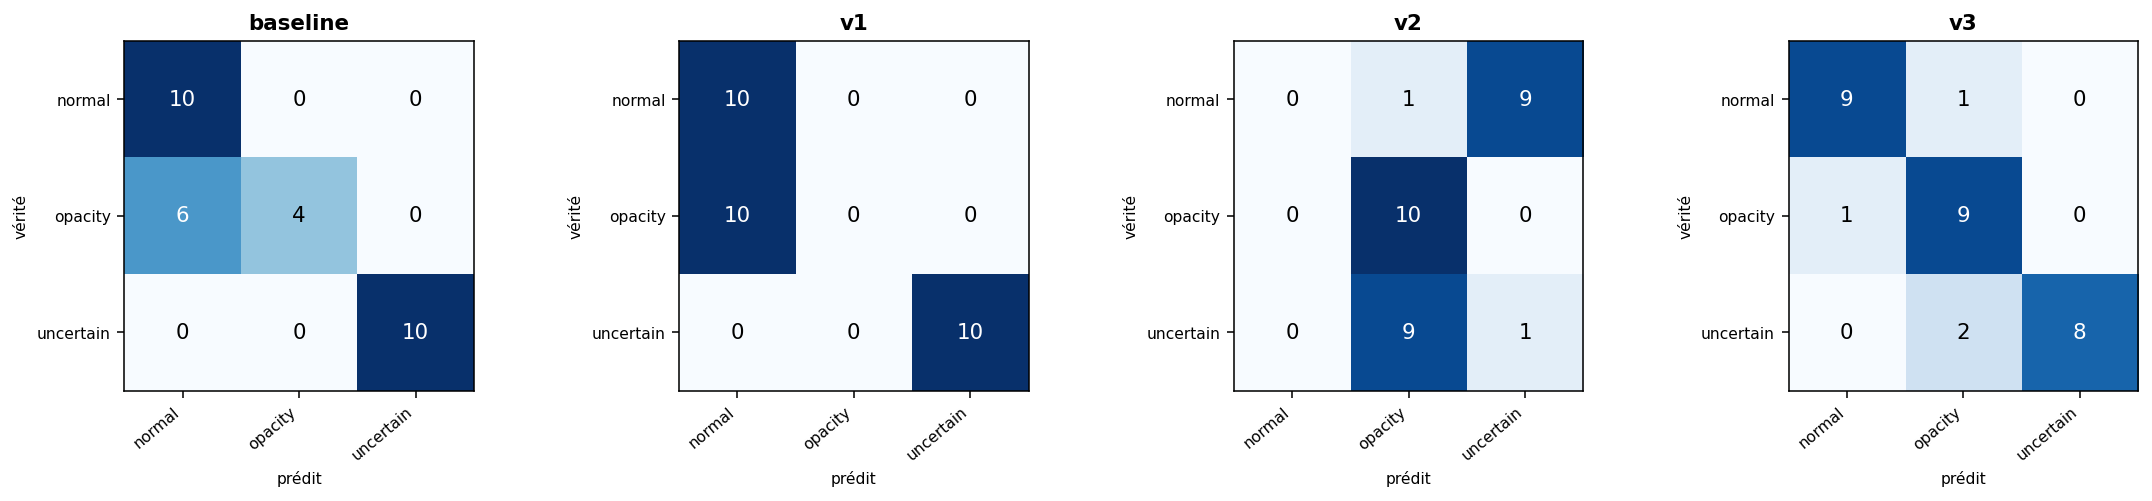
\includegraphics[width=\textwidth]{figures/confusion_matrices.png}
\caption{Matrices de confusion des quatre versions (lignes = vérité, colonnes = prédiction).
On lit directement les deux modes d'échec (v1 : tout en \texttt{normal} ; v2 : rien en
\texttt{normal}) et la convergence de la v3.}
\end{figure}

\begin{keybox}
\textbf{Leçon d'ingénierie.} L'arc baseline $\rightarrow$ v1 $\rightarrow$ v2 $\rightarrow$ v3
montre qu'un prompt « de sécurité » plausible a silencieusement dégradé la sûreté clinique. La
fluidité du texte produit ne garantit pas la correction : seule la mesure systématique a permis de
diagnostiquer chaque échec et de converger vers un compromis défendable.
\end{keybox}

\section{Évaluation et analyse d'erreurs}

\subsection{Protocole et métriques}
L'évaluation calcule exactitude, macro-F1, sensibilité (\texttt{suspected\_opacity}), spécificité
(\texttt{normal}), taux de JSON valide, taux d'avertissement, taux d'incertitude et latence. Les
runs sont journalisés en SQLite. La commande \texttt{python eval/run\_evaluation.py --mode
improved\_v3} rejoue l'ensemble sur CPU.

\subsection{Taxonomie d'erreurs}
\begin{table}[h]
\centering
\renewcommand{\arraystretch}{1.2}
\begin{tabular}{ll}
\toprule
\textbf{Code} & \textbf{Signification}\\
\midrule
FN & Faux négatif --- anomalie présente prédite \texttt{normal}\\
FP & Faux positif --- image normale prédite suspecte\\
UA & Incertitude acceptable / cas ambigu forcé\\
JF & Erreur de format JSON\\
HT & Hallucination textuelle (signe non visible mentionné)\\
\bottomrule
\end{tabular}
\caption{Taxonomie utilisée dans le registre d'erreurs.}
\end{table}

\subsection{Registre d'erreurs (extrait)}
Le registre complet (\texttt{eval/error\_register.csv}) documente 10 cas commentés : les 4 erreurs
résiduelles de la v3 et 6 cas d'ablation illustrant les modes d'échec de v1 et v2. Les erreurs
résiduelles de la v3 sont la tension naturelle du compromis : une opacité encore manquée
(\texttt{CXR\_SYN\_017}), une image normale sur-signalée (\texttt{CXR\_SYN\_010}) et deux cas
ambigus poussés vers \texttt{suspected\_opacity} plutôt que \texttt{uncertain}.

\section{Éthique, sécurité et limites}

\subsection{Garde-fous fonctionnels}
Chaque sortie passe par des garde-fous : validation stricte du schéma JSON, avertissement
non clinique forcé sur 100\,\% des sorties, règle d'incertitude (repli vers \texttt{uncertain} en
cas de doute ou de faible confiance), et journalisation des prompts, modèles, sorties et latences.

\begin{warnbox}
\textbf{Avertissement obligatoire (présent dans l'UI, le JSON, le README et la soutenance) :}\\
Prototype pédagogique. Non destiné au diagnostic. Validation par un professionnel qualifié requise.
\end{warnbox}

\subsection{Limites documentées}
\begin{itemize}[leftmargin=1.4em]
\item \textbf{Données synthétiques.} Les images ne sont pas cliniques ; les scores ne mesurent que
le pipeline et la sensibilité aux prompts.
\item \textbf{Petit échantillon.} 30 images, 10 par classe : les valeurs sont illustratives, pas
statistiquement robustes.
\item \textbf{Confiance non calibrée.} Le modèle produit des valeurs de confiance peu variées
(souvent 0,95 ou 0,20), non fiables comme probabilités.
\item \textbf{Sensibilité au prompt.} Démontrée quantitativement : un changement de formulation
fait varier l'exactitude de 36,7\,\% à 86,7\,\%.
\item \textbf{Validation indépendante requise} pour tout usage réel.
\end{itemize}

\section{Références techniques et licences}

\begin{keybox}
\textbf{Modèle} \texttt{google/medgemma-4b-it} (instruction-tuned).\\
\textbf{Architecture} variante Gemma~3 avec encodeur d'image SigLIP pré-entraîné sur des données
médicales dé-identifiées, dont des radiographies thoraciques.\\
\textbf{Accès} modèle sous accès contrôlé (\emph{gated}) sur Hugging Face ; connexion et
acceptation des conditions requises.\\
\textbf{Licence / conditions} \emph{Health AI Developer Foundations terms of use}.\\
\textbf{Restrictions d'usage} recherche et éducation ; non destiné au diagnostic ; non validé comme
dispositif médical.\\
\textbf{Code du dépôt} licence MIT ; les datasets et modèles externes conservent leurs licences
propres.
\end{keybox}

\vspace{0.4cm}
\noindent Conformément au cahier des charges, aucune donnée patient réelle n'a été utilisée ni
commitée. Les extensions avancées (LoRA/QLoRA, MIMIC-CXR, CheXpert) n'ont pas été mobilisées ;
elles sont documentées comme pistes \texttt{COULD} nécessitant un dataset réel sous accès contrôlé.

\section{Conclusion}
Le prototype démontre une méthode plutôt qu'une prouesse : périmètre restreint, baseline
reproductible, garde-fous, évaluation chiffrée et analyse d'erreurs. Son apport principal est
l'itération mesurée des prompts, qui établit empiriquement que la prudence \emph{doit être
mesurée} et non supposée. La version finale (v3) est prudente, défendable et documentée --- ce que
le cahier des charges valorise davantage qu'une solution spectaculaire mais infalsifiable.

\end{document}
